\section{Validation of the simulation}
In \cref{sec:validation} I presented two methods of validating the simulator. The intuitive and analytical methods. The intuitive validation I have already explained there. The results of the intuitive validation I did I believe show that the simulator at least "acts right". Any flaws that it may have are not so obvious that they are visible without analysis. I will here try to do some further analysis here below of the tension data. 

\subsection{Tension data}
Looking at the results from \cref{tab:tension} and \cref{fig:tensions}, I believe the simulator can be called valid for this use-case. In all cases, except for the fastest one, the simulated tension falls between or below the assumed drag values.  The deviations from the calculated values are shown in \cref{tab:deviation}. The cause of the deviations are likely because of the way I've done the calculations; ignoring tumbling and using a "best guess" value for the drag coefficient. Looking at the actual simulation for the highest speed I can confirm that my assumptions will be completely off, as the ROV in that case is practically surfaced as it is dragged behind the surface vessel, see \cref{fig:dragged}. The cross-sectional area used in the calculations will be far off from the real values here, as it's almost the "top" surface of the ROV that's facing the direction of travel. Another point to note is that at these high speeds the surface vessel tips so far forward it gets caught up by the hydrodynamic forces at the water's surface and flips over. I believe this happens because the tether is not perfectly centred on the body of the surface vessel, but it is also somewhat a bad sign for such high speeds with this vessel. It indicates that stability analysis at different speeds should be performed. When it comes to the vessel's tipping at higher speeds and validity of the results: the velocity with which the tether is dragged is set and independent of the surface vessel. The vessel is being given a speed with infinite acceleration and is simply along for the ride.

\begin{figure}
	\centering
	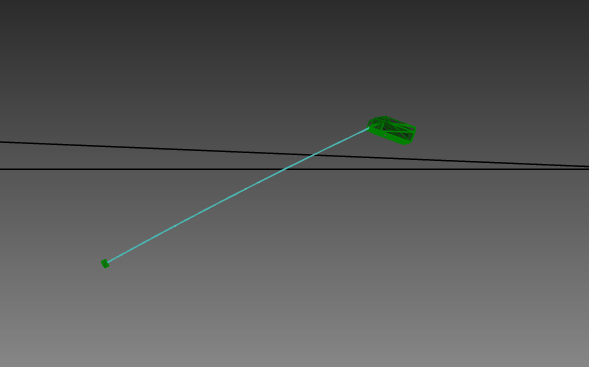
\includegraphics[width=0.6\textwidth]{dragged}
	\caption{The ROV shown dragged behind the surface vessel at \(v=5\frac{m}{s}\)}
	\label{fig:dragged}
\end{figure}

What this dragging simulation tells us is that at this depth, the ROV is not usable. This can be a useful tool to gauge what speeds the surface vessel will be able to move without adversely affecting the ROV underwater. For example, in \cref{fig:notstraight} the surface vessel is also moving at \(v=5\frac m s\), but the ROV is not as affected because the tether damps more when it is longer. The results also show that the analytical method provides an overestimate for the force that the tether will be required to endure under low-speed conditions. This can be used as a tool to find suitable tether materials.

Further, looking at the two first simulation cases they show a very close relationship with the analytical method. At \(v=0\), the simulator has 2.4\% less tension than the analytical method expects. This can be because the tether has an impact. If the tether is slightly non-buoyant, the ROV would experience a smaller tension than the surface vessel. This is because the surface vessel would carry the weight of both the tether and the ROV, while the ROV will not "notice" the tether in its connection.

Looking at \(1\frac{m}{s} \leq v \leq 4\frac m s\) the tension is lower than calculated. Looking at the graphical output of the simulation, the suspicion mentioned in \cref{sec:anal} is confirmed and the ROV is indeed tumbling a bit, presenting a sharp angle towards the direction of travel instead of the blunt front. This would lower the coefficient of drag significantly. For instance, an angled cube, presenting a corner towards the stream rather than a face, has \(C_D = 0.80\) compared to a face-on cube with \(C_D=1.05\). 

All in all, I believe the differences in results between the analytical method and the simulated method can be seen as a combination of tumbling and angling. By angling I mean presenting a sharper angle towards the stream, and by tumbling I mean presenting the larger top face instead of the smaller front face. Angling would decrease the coefficient of drag while tumbling would increase the forward facing area. I believe these two effects explain the discrepancies seen. Further, I believe that the simulator provides more accurate data than the analytical method could as I have used it. I believe this because the simulator is able to account for angling, tumbling and other effects which are much harder to implement in the closed-form equations I've used. 

\section{Use as a rapid prototyping tool}
The simulator shows a lot of promise as a rapid prototyping tool. As it stands at time of writing, it is fairly easy to configure. Changing for example initial conditions, depths of water/length of cable or the type and tuning of controller is very simple. Configuring the seastate is somewhat more complex as it's necessary to describe an elevation function for the sea surface. Currents and waves are not currently implemented, but waves should be fairly simple to implement given an elevation field, and judging by the rest of the framework I doubt currents are much more difficult.AGX allows for currents using the \texttt{WaterFlowGenerator} interface. 

\section{Future work}
Currently only the surface vessel has a control system implemented and this control system is a waypoint style system. The ROV is only a hanging weight as implemented right now. In the final implementation of the Plan Sea project, it's likely that one of the vessels will be actively following the other to allow for the desired range of motion or lifting strength. Thus further development on the control side of the simulator is necessary. 

The tether connecting the surface vessel and the ROV is currently a fixed length. AGX does have methods of simulating winches, including their internal forces, required torques and other elements. This implementation should be considered a high priority to make the simulation closer to reality and allow for more dynamic states to be simulated. 

Further, there are no environmental effects as the simulator stands today. Implementing especially currents would be essential to getting a model that can be instructive about the real-life applicability of the controllers designed. Waves would also be important to implement, along with a heave-compensation system to allow the ROV to maintain altitude even as the surface vessel is moving vertically. 

The simulator right now requires a knowledge and understanding of both Python and AGX to configure and run. It would be nice if in the future it is possible to configure basic functions of the simulator through a graphical user interface as opposed to through code. I believe this should be a lower priority to implement, as currently the simulator is a development tool, but it would be nice to have. 

Another nice-to-have is a better model of the surface vessel and the ROV. More detailed models would allow for a more accurate hydrodynamic simulation to be run. Higher detail would also increase the complexity of the model though, so it should only be implemented to a certain point. I believe that better models should also be considered a low priority, as the approximations taken right now are likely accurate enough, within one order of magnitude or so. 

For my Master's thesis, I would like to work further on this simulator to create a well functioning control system and then apply it to the real-life vessel and ROV. I would implement some of these changes, as well as deal with the physical modifications of the real-life vessel and ROV. 